\documentclass{acm_proc_article-sp}
\usepackage[utf8]{inputenc}
\usepackage{graphicx}
\usepackage[plain]{algorithm}
\usepackage{algpseudocode}
\newenvironment{Figure}
  {\par\medskip\noindent\minipage{\linewidth}}
  {\endminipage\par\medskip}

\begin{document}
\graphicspath{{figures/}}

\title{“Starter kit for smart buildings”}
\subtitle{Pervasive Computing : Selected Topics Project}

\numberofauthors{2} %  in this sample file, there are a *total*
% of EIGHT authors. SIX appear on the 'first-page' (for formatting
% reasons) and the remaining two appear in the \additionalauthors section.
%
\author{
\alignauthor 
  Aebischer Nadia
  \affaddr{Department of Informatics}\\
  \affaddr{University of Fribourg}\\
  \affaddr{1700 Fribourg, Switzerland}\\
  \email{nadia.aebischer@unifr.ch}
\alignauthor 
  Luyet Gil
  \affaddr{Department of Informatics}\\
  \affaddr{University of Fribourg}\\
  \affaddr{1700 Fribourg, Switzerland}\\
  \email{gil.luyet@unifr.ch}
}
\date{\today}
% Just remember to make sure that the TOTAL number of authors
% is the number that will appear on the first page PLUS the
% number that will appear in the \additionalauthors section.
\maketitle
\begin{abstract}
The goal of this report is to describe an easy way to integrate a basic pervasive system into an already built house/building. 
The system should be cheap and easy enough to integrate and to operate so it could be used by the masses as a starter kit for smart buildings. 
The report will be based on the data analysis and the context of use of this system. 
Especially about the central unit managing the whole house.
\end{abstract}
\section{Introduction}
\subsection{Smart building description}
A smart building is by definition a building enhanced by the technology that is managing it. 
Generally the technology used is splitted into four parts. 
First, we have the sensors that collect data and allow to have an understanding on what is going on outside or within the house. 
The second part is the network that allows to spread the data collected by the sensors and to eventually activate the actuators if needed. 
The third part is the managing unit that allows to gather data and infer knowledge about the environment and thus either show the data to the user or activate actuators to change the user’s environment. 
The last part is the data visualisation that allows the user to interact with the data.
This structure follows the given standard loop of a pervasive system shown in Figure \ref{loop}.
%++++++++++++++++++++++++++++++++++++++++++++++++++++++++++++++++++++++++++++
				\begin{figure}[htb]
  				\begin{center}
    				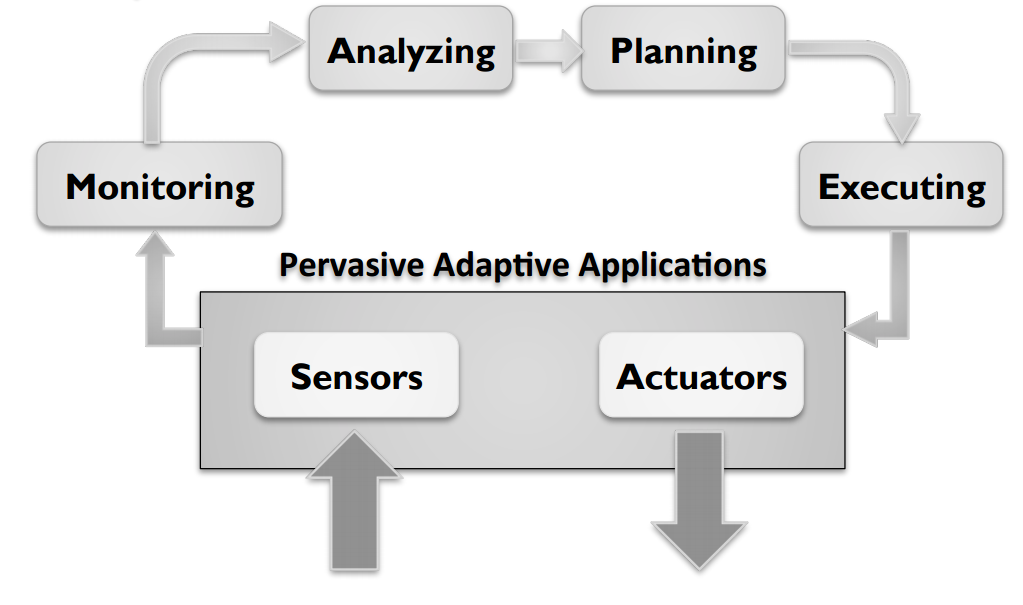
\includegraphics[width=\linewidth]{loop}
    				\caption{Pervasive system loop \label{loop}}
  				\end{center}
				\end{figure}
%++++++++++++++++++++++++++++++++++++++++++++++++++++++++++++++++++++++++++++
\subsection{Aim of the project}
The basic aim of the project is simple.
We would like to produce a simple to use and to integrate system that would allow to enhance an already built building to a smart building. 
This system should be relatively cheap and should involve the least possible physical changes in the house (e.g. destroying walls).
This means that it has to be based on cheap and already existing means and be a sort of “do-it-yourself” kit.
\section{House description}
\subsection{Context of use}
We are going to consider a small building with a dozen of individual apartments. 
Each apartment would have four rooms, each one having one light and one window with an electric sunblind. 
In such a configuration it is usual to split the power supply into so call groups. 
Each group has its own electrical phase. 
For a standard four rooms apartment (one kitchen, three rooms and one bathroom) we would have three or four groups: one managing the kitchen, one managing the bathroom and one or two groups for the other rooms. 
The building has a central water heater, separated electric meters per apartment and an individual thermostat per apartment. 
A central electrical panel is available for the whole building. An indoor parking space in common with an electric door that is activated by a remote controller is also considered.
\subsection{What could be automated}
Sunblinds are opening or closing automatically by checking the sunlight and time. 
For example if it's sunny the sunblinds will be closing. The same way, at night, they should be closing to protect our privacy.
The temperature of the apartment can also be automated. For example we can set the temperature we want to have in the apartment, 
and if the actual temperature is below or above the default one we set, the system will change the thermostat accordingly. 
We can also imagine a way to infer if somebody is going to be there soon or not and raise more or less fast the overall temperature. 
This inference can be computed according to the presence of people in the house by reading the presence sensors. 
For example, if somebody is never present during the weekends then the central unit should over the time learn that fact and thus it will heat the apartment in order to saving energy.
The lights can also be automated by detecting the presence of people in a room.
RFID tags linked with cars could be used to open the parking space doors.
Of course, these automated behaviors can be stopped by the user if he doesn't want it to be performed. 
To do so, the user can access the central unit via a web interface and change the behavior the way he want at all times.
%++++++++++++++++++++++++++++++++++++++++++++++++++++++++++++++++++++++++++++
				\begin{figure}[htb]
  				\begin{center}
    				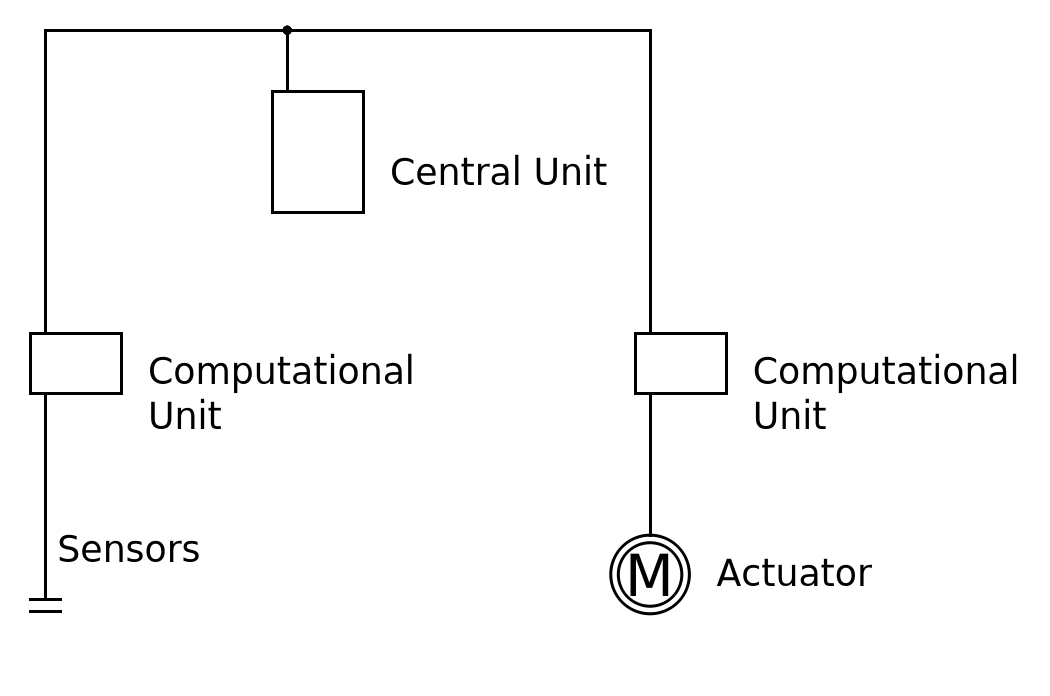
\includegraphics[width=\linewidth]{architecture}
    				\caption{System architecture \label{architecture}}
  				\end{center}
				\end{figure}
%++++++++++++++++++++++++++++++++++++++++++++++++++++++++++++++++++++++++++++

\section{Sensors}\label{sensors_section}
In this section, we will briefly talk about the different sensors that our Central Unit will deal with. 
We are not going into too much details as it is not our main subject for this project.
\subsection{Sensors architecture}
The communication between the components are achieved by WiFi or over the electrical network in case the WiFi is not reachable. 
Communication over the electrical network can achieve a very fast connection speed between the components, up to 1200 Mbits/s\footnote{http://www.devolo.com/en/Products/dLAN-1200+}. 
This means that theoretically preprocessing of sensors data is not needed but for utility reasons we will preprocess the data before reaching the Central Unit.
Each sensor is connected to a light computer, typically a Raspberry Pi could work but we can imagine an even less powerful one for small tasks. 
This light computer will preprocess the raw sensor data and play the role of the interface between the sensor and the Central Unit. 
This interface is needed in case of multiple types of sensors. By changing the sensors, one could simply apply a patch to the small computer (even via the Central Unit) and resolve compatibility issues. For the rest of this report, we'll call this kind of light computer linked to sensors or actuators, a \textit{computational unit}.
This interface used is a simple HTTP based communication via POST with a specific XML-based body very similar to the SOAP protocol. 
This produce a simple Service-Oriented Architecture (SOA) to access the data. 
Here is an example:
\begin{verbatim}
POST address 
  <MESSAGE>
    <TYPE>(alert|event|failure|do|synch)</TYPE>
    <FROM>(sensor_id|central_unit)</FROM>
    <CONTENT/>
  </MESSAGE>
\end{verbatim}
Where the \texttt{TYPE} denotes an alert, an event or even a failure for example. 
The \texttt{FROM} and \texttt{CONTENT} parts deals respectively with the author of the message and the actual meaning of the message. 
A typical proximity sensor message would look like the following (it's the computational unit that will send the message, and not directly the sensor):
\begin{verbatim}
POST central_unit 
  <MESSAGE>
    <TYPE>event</TYPE>
    <FROM>sensor_id2345</FROM>
    <CONTENT>distance:'2.34m'</CONTENT/>
  </MESSAGE>
\end{verbatim}
A typical message sent by the Central Unit to open a door would be:
\begin{verbatim}
POST address_of_door_actuator
  <MESSAGE>
    <TYPE>do</TYPE>
    <FROM>central_unit</FROM>
    <CONTENT>door[0]:'open'</CONTENT/>
  </MESSAGE> 
\end{verbatim}
\subsection{Location}
The locations of the sensors depend of the type of sensor. Here is the list of the sensors we are going to consider:
\begin{description}
 \item[Luminosity sensor] - inside each room and outside at each frontage of the house.
 \item[Presence sensors] - around the lights and the doors.
 \item[Temperature sensors] - one inside at the center of the apartment and another outside.
 \item[Energy consumption sensor] - after the electric meter.
 \item[Water consumption sensor] - before the water inlet.
 \item[Water temperature sensor] - after the water heater.
 \item[RFID readers] - for cars around the garage doors.
\end{description}
We also consider actuators, the list of them is given here:
\begin{description}
 \item[Sunblinds actuators] - to open and close sunblinds.
 \item[Light actuators] - to switch the lights on and off.
 \item[Thermostat actuator] - to change the house temperature.
 \item[Automatic garage door opener] - to be linked with the RFID reader.
\end{description}
This part is not really important for the scope we choose to aim our report, but this should be at least mentioned because it lists which sensors we are going to consider and we are receiving data from in order to form a context, and also on which actuators the Central Unit can send message to change the environment.
\section{Central Unit}	
The Central Unit is the main part of this architecture and the scope of this report. 
This Central Unit depends on several topics as its own architecture, the sensors data coming in, 
the actuators it has to interact with its environment and of course its standard interface with the user.
\subsection{Architecture of central unit}
The architecture itself has no specific requirement. 
We can choose whatever we want, here we might focus on a standard Linux distribution as Ubuntu without any graphical environment as the only interaction we have will be via a web interface discussed later. 
Furthermore the computation needed is not too high as the preprocessing of the sensor is done on the sensor side with light computer as discussed earlier. 
The computer should also be running 24/7 and thus the computer has to have a low consumption. A light computer as a Raspberry Pi might be enough.
\subsection{Sensor fusion}
The sensors fusion is performed to produce a context. A context is the actual state of an entity such as a room or a person. 
In this report we need to know exactly which kind of contexts we are going to consider to know exactly which sensor data has to be aggregated to produce the actual state of a room for example. 
The aggregation itself will be done in such a way that sensors failure could be minimized.
A standard way to do this can be done via computing a mean value of the last dozen of incoming values and use this mean as the incoming sensors value.
\subsubsection{Sensors message synchronization}
As some sensors output can be asynchronous, e.g. if we take the presence sensor it could output each time it detects a presence, we need to introduce some kind of synchronization protocol similar to the WiFi communication protocol.
Each sensor we have is connected to a little computer used for preprocessing sensor inputs, this allows us to synchronize the data flow by offering time windows management.
This kind of management is usually done by either giving a time frame by sensor or allowing one big time frame to allow each sensor to send periodically during a certain amount of time.
The second option will be taken here but we might introduce a little modification. 
The size and the exact beginning of this time frame is not fixed but we introduce here Ready-To-Send (RTS) messages similar to WiFi collision avoidance protocol.
Each time the Central Unit has finished to infer all the contexts it sends a RTS message to all the sensors to notify them that they can send their data.
Such a message would look like the following.
\begin{verbatim}
POST address_of_sensor 
  <MESSAGE>
    <TYPE>synch</TYPE>
    <FROM>central_unit</FROM>
    <CONTENT>RTS</CONTENT/>
  </MESSAGE> 
\end{verbatim}
During the time between two RTS messages sensors are able to aggregate their sensors value to give a mean value of them.
As the sensors are now synchronized we need to infer contexts from their data.
\subsubsection{Communication}
We already saw how each computational unit will send data to the Central Unit. Now, we want to make sure that this communication happens smoothly. 
When the computational unit sends a message to the Central Unit, the latter must confirmed that it receives the message, and if it's not the case, 
the computational unit will send again the same message. 
This statement is also true for the other way around. 

\subsubsection{Context inference}
Inferring contexts depends on the states from several sensors. In this part of the report we list the contexts choosen and how to obtain them.
A certain context may depend on several subcontext or states, 
e.g. the lightning state of a room may depend on the outside lightning, the state of the lights of the room and the states of the sunblinds.
\subsubsection*{The lightning state of the room}
 This context is composed of distinct contexts, the lightning of the room and the outside environment \textbf{("dark" or "lighted")} and the sunblinds states \textbf{("open" or "closed")}. 
 Of course those contexts are inferred by using multiple sensors input, e.g. multiple sunblinds implies multiple sunblinds states that will be summed. But we will not extend the description of such details.
 The lightning state of the room itself may be described as ("dark" or "naturally lighted" or "artificially lighted").
 Knowing the lightning state of the room in combination with the time of the day will be useful in order to know if the lights must be turned on or off, and if the sunblinds must be opened or closed. Now we are going to consider the states \textbf{dark} and \textbf{lighted}. These two states can be determined thanks to the luminosity sensors present inside each room and a arbitrarily threshold that the user can change via the web interface of the Central Unit.
 \begin{description}
  \begin{algorithm}
  \begin{algorithmic}
    \If {\textit{lightning of the room} $\leq$ lightning\_threshold}
      \State $state\gets$ dark
    \Else
      \State $state\gets$ lighted
  \EndIf
  \State \textbf{return} $state$
  \end{algorithmic}
  \end{algorithm}
\end{description}
We can then also differentiate between natural and the artificial lighting by the following inference. For this case, we are also considering the states of the lights switches known by the Central Unit:
\begin{description}  
  \begin{algorithm}
  \begin{algorithmic}
    \If {\textit{lightning of the room} > lightning\_threshold}
      \If {\textit{outside lightning} > lightning\_threshold $\land$ \textit{lights of the room} = off $\land$ \textit{sunblinds} = open}
	\State $state\gets$ naturally lighted
      \ElsIf {\textit{outside lightning} = dark}
	\State $state\gets$ artificially lighted
      \EndIf
    \EndIf
  \State \textbf{return} $state$
  \end{algorithmic}
  \end{algorithm}
\end{description}
 \subsubsection*{The occupation of the room}
 In order to determine the actual occupation of the room (\textbf{"empty" or "occupied"}), we need to merge the inputs of the presence sensors of the room.
 Each presence sensor can determine if something moves around it. 
 So if someone enters the room the sensors will determine that the room is occupied, and once the person stays still in the room the sensors should not determine that the room is empty. 
 To solve this the sensing should stop or be ignored by the Central Unit for a certain amount of time set by the user.
 This is a typical event message that will be sent to the Central Unit:
 \begin{verbatim}
POST central_unit 
  <MESSAGE>
    <TYPE>event</TYPE>
    <FROM>sensor_id</FROM>
    <CONTENT>presence:('true'|'false')</CONTENT/>
  </MESSAGE> 
\end{verbatim}
Those sensors inputs are merged to produce a single state of the room.
If $S$ is the set of sensors used, then the state is infered by the following equations:
 \begin{description}
 \begin{algorithm}
  \begin{algorithmic}
    \If {$\underset{s \in S}{\lor} s_{state}$ = true}
      \State $state\gets$ occupied
    \Else
      \State $state\gets$ empty
  \EndIf
  \State \textbf{return} $state$
  \end{algorithmic}
  \end{algorithm}
 \end{description}
 \subsubsection*{The actual weather state inside and outside}
 This context depends on many different sensors input and merging.
 The first subcontext to determine how the temperature state is outside and for each room is as (\textbf{"cold", "comfortable" or "hot"}). 
 Those terms are based on a user-determined threshold. This threshold can be set by the user via the web interface of the Central Unit.
 Each subcontext can be infered by using data provided on the Internet or by using outside temperature sensors.
 If $S$ is the set of sensors used outside or inside then the temperature is determined by the following inference.
 \begin{description}
 \begin{algorithm}
  \begin{algorithmic}
  \State $temp\gets \frac{\underset{s \in S}{\sum} s_{value}}{|S|}$
   \If {$temp \in range_{hot}$}
    \State $state\gets$ hot
   \ElsIf {$temp \in range_{comfort}$}
    \State $state\gets$ comfort
   \ElsIf {$temp  \in range_{cold}$}
    \State $state\gets$ cold
   \EndIf
  \State \textbf{return} $state$
  \end{algorithmic}
  \end{algorithm}
  \end{description}
 The precipitations states (\textbf{"rainy" or "dry"}) can be infered by using values retrieved over the Internet.
  \subsubsection*{Which part of the day is it?}
  The actual date and time is enough to infer such an information.
  The part of the day can be \textbf{"morning", "noon", "afternoon", "evening" or "night"}
 \subsubsection*{Is a car waiting at the garage doors ?}
 If an authorized car approches the RFID reader then the door can be opened.
 The message sent by the RFID reader has the following form:
  \begin{verbatim}
  POST central_unit 
  <MESSAGE>
    <TYPE>event</TYPE>
    <FROM>RFID_reader</FROM>
    <CONTENT>
      presence:('true'|'false'),
      car:('allowed','forbidden')
    </CONTENT/>
  </MESSAGE> 
\end{verbatim}
If a car with a RFID tag approaches the RFID reader then the presence field turn to "true". If the tag is authorized then the car field turn to "allowed".
 \subsubsection*{What is the actual consumption of the whole building ?}
 This context might be inferred by using the three following sensors, the energy consumption sensor which measures the electric consumption, 
 the water consumption and temperature sensors that measure the current state of the water status of the house.
 Those sensors can be used to infer two subcontexts that are the current status and the overall status.
 The current status display the consumption of the building or the apartment in real time.
 The overall status can be computed by aggregating the sensors values and store them into a small database.
 The user can then access those values over the web interface provided by the Central Unit.

We choose those six contexts because they cover many facets of the Central Unit (web interface, data aggregation or even information retrival over the Internet).

\subsection{Web-based manual controller}
%for mobile + desktop + over Internet
We think that our system must have an interface in order to offer a manual management of it.
As the transmission of the data sensors is based on the standard HTTP protocol we can deduce that the network also support web-based application.
Providing a web-based interface can be useful because with nowadays technologies we can provide the same website or web application for mobile and desktop devices with adapting templates.
This precision is important because smartphones are widely used, and thus they can be used to access the Central Unit more easily. 
Furthermore using a web-based application with a good authentication protocol, such as HTTPS, can make the interface available over the Internet.
This gives more freedom to the users, as they can control their homes at work or switching off the lights forgotten in the morning on the go.

%interface used for conrol (lights)
As suggested this interface should be used to also control the automation of the building.
For each room the user can choose to switch the lights on or off and to open or close the sunblinds.
The user can fix the temperature he wants to maintain in the apartment and he can activate or not the detection of presence (i.e. if the user is not at home but there is a cat, it can be convenient to deactivate the detection of presence).
As we saw earlier, the lights, sunblinds are automatically controlled by the Central Unit depending of the informations received by the sensors. But, it can be handy for the user to take over this control and changing the actual work flow of the Central Unit.
A grid-based (4 $\times$ 5) design (i.e. iOS or Android applications screen) should allow the user to quickly choose among lights, sunblinds, temperature or detection of presence controls, then a room and finally he can stop the actual behaviour and change it. By doing so, the Central Unit will not automate the behavious of the particular material that has been changed until the user tell it by click on a button that will "reactivate" the automation.

%stats presentations
The interface must also display informations that are gattered by the system to monitor the building activity.
Those statistics as the water or electricity consumption might be displayed to the user into understandable graphics.
These statistics can then help the user to change the way he consumes those different resources or to detect if something is off (i.e. a water leak results in higher consumption of water).

%failure presentations
The web-based controller can also be used in case of failure by displaying the exact location or type of failure and allow a more efficient reparation and diagnostic.
In our grid-based template, one element will give access to a list of failure items (most recent failure will appear first).
The possible failures are discussed in Section \ref{failure_handling}.
%++++++++++++++++++++++++++++++++++++++++++++++++++++++++++++++++++++++++++++
				\begin{figure}[htb]
  				\begin{center}
    				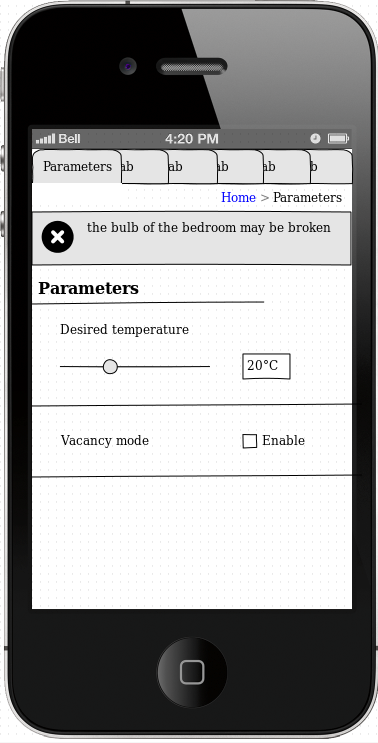
\includegraphics[width=5cm]{mockup}
    				\caption{Web interface mockup for smartphone\label{mockup}}
  				\end{center}
				\end{figure}
%++++++++++++++++++++++++++++++++++++++++++++++++++++++++++++++++++++++++++++


\section{Actuators}
Admit now that each context has been computed by using the sensor data.
We must now describe how an actual context combined with new sensors data coming in will react. 
This is what we call \textit{'coordination'}. 
Our entities are here the central unit, the actuators and the sensors.
The interactions are done via the messages sent to each others and the rules are simply a list of allowed interactions.
We can list all the possible interactions and the messages sent by the Central Unit to the actuators.
The evolution of the system will derivate from this simple set of rules.
Here we only gives a few examples for the messages as their are very similar.
We can also add that after this definition of coordination the message coordination explained in section~\ref{sensors_section} can be seen as time synchronization between the entities.
\begin{description}
% \begin{description}
%  \begin{algorithm}
%   \begin{algorithmic}
%    \If {\textit{somebody enters the room}$\land$ \textit{room is dark}}
%     \State switch lights on
%    \EndIf
%   \end{algorithmic}
%   \end{algorithm}
%   \end{description}
% \begin{description}
 \item[Do] activate lights \textbf{if} somebody enters the room $\land$ room is dark\\
 \begin{verbatim}
  POST light_switch_id 
  <MESSAGE>
    <TYPE>do</TYPE>
    <FROM>central_unit</FROM>
    <CONTENT>light:'on'</CONTENT/>
  </MESSAGE> 
\end{verbatim}
 \item[Do] deactivate lights \textbf{if} room is empty $\land$ room is lightened
 \item[Do] reduce heating \textbf{if} room is usually empty for a quite long period $\land$ nobody is inside.\\
 The "quite long period" is a period of time that can be manually set by the user or this information can be infered by the Central Unit thanks to past data if they exist.
 \begin{verbatim}
  POST thermostat 
  <MESSAGE>
    <TYPE>do</TYPE>
    <FROM>central_unit</FROM>
    <CONTENT>set_temp:'value'</CONTENT/>
  </MESSAGE> 
\end{verbatim}
 \item[Do] reduce heating \textbf{if} outside temperature > comfort temperature $\pm$ threshold
 \item[Do] augment heating \textbf{if} temperature < comfort temperature $\pm$ threshold.
 \item[Do] open doors \textbf{if} car is at the parking doors $\land$ door closed.
 \item[Do] close the doors \textbf{if} timer for doors is over $\land$ no car at the parking doors.\\
 \begin{verbatim}
POST door_actuator
  <MESSAGE>
    <TYPE>do</TYPE>
    <FROM>central_unit</FROM>
    <CONTENT>door[0]:'open'</CONTENT/>
  </MESSAGE> 
\end{verbatim}
 \item[Do] close sunblinds \textbf{if} sunblinds open $\land$ lightning outside < lightning\_threshold $\land$ part of the day = ’evening $\lor$ night’.
 \item[Do] open sunblinds \textbf{if} sunblinds closed $\land$ part of the day != ’evening $\lor$ night’ $\land$ someone enters the room.
\end{description}
\subsection{Actuators architecture}
All our actuators depend on electrical input to work. The main idea of performing remote activation of actuators depends on a single element that we will name "Smart Switch".
A smart switch is a standard switch (on-off) button that can be activated by a simple computer and that will allow or not electricity to pass.
  %We can found many example of those switch over the Internet.
We then can specify each use of those switches.
We are going to specify here two types of lightning actuators and the doors actuators.
\subsubsection{Lightning}
The first type of lightning switch is called "schema 0" and is the most simple case of switch possible.
Its structure is shown in Figure \ref{schema0}.
In that case it is possible to let the actual wire structure as it is and only replace the classical switches by our smart switches.

%++++++++++++++++++++++++++++++++++++++++++++++++++++++++++++++++++++++++++++
				\begin{figure}[htb]
  				\begin{center}
    				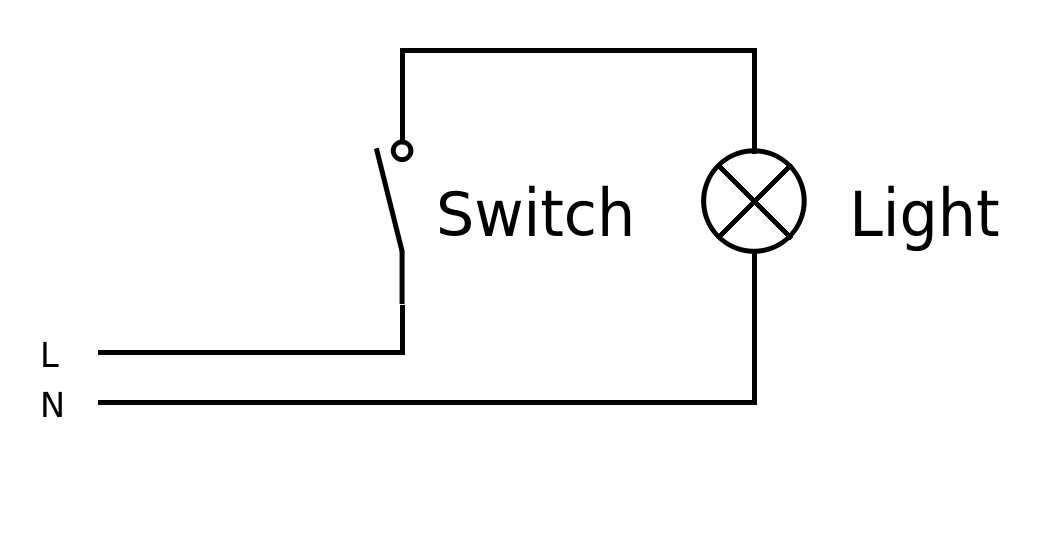
\includegraphics[width=\linewidth]{schema0}
    				\caption{Schema 0 \label{schema0}}
  				\end{center}
				\end{figure}
%++++++++++++++++++++++++++++++++++++++++++++++++++++++++++++++++++++++++++++

A problem occurs when dealing with more complex wired structures. We here only discuss of the "shema 3" type that allows to control one single light
with two switches. Its structure is shown in Figure \ref{schema3}.
%++++++++++++++++++++++++++++++++++++++++++++++++++++++++++++++++++++++++++++
				\begin{figure}[htb]
  				\begin{center}
    				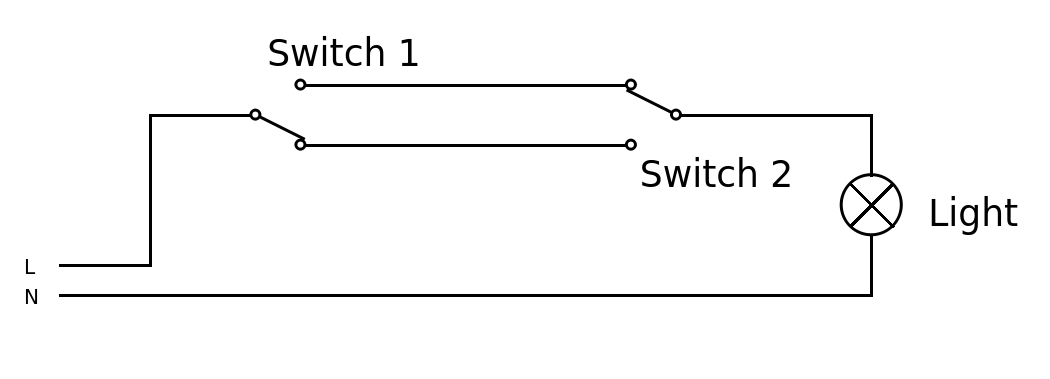
\includegraphics[width=\linewidth]{schema3}
    				\caption{Schema 3 \label{schema3}}
  				\end{center}
				\end{figure}
%++++++++++++++++++++++++++++++++++++++++++++++++++++++++++++++++++++++++++++
Here the problem is that the structure is now composed of multiple wire.
But we can solve this situation by allowing each light actuator unit to send a message to the other units that compose also the same lightning structure.
Each time a switch is ordered to be turned "on" or "off" it relays the same message to all the others concerned light actuators.
We can then remove wires and keep only one direct link between all switches as shown in Figure \ref{new_schema3}
%++++++++++++++++++++++++++++++++++++++++++++++++++++++++++++++++++++++++++++
				\begin{figure}[htb]
  				\begin{center}
    				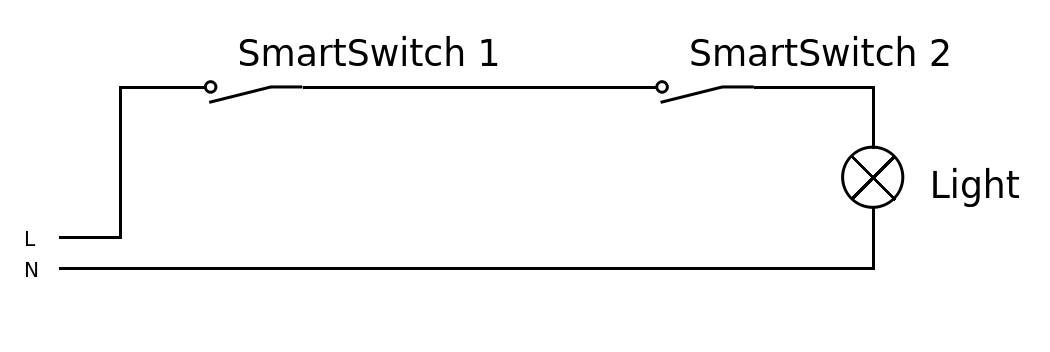
\includegraphics[width=\linewidth]{new_schema3}
    				\caption{Smart schema 3 \label{new_schema3}}
  				\end{center}
				\end{figure}
%++++++++++++++++++++++++++++++++++++++++++++++++++++++++++++++++++++++++++++
All other variants of "schema" are "schema 3" linked with special switches. This means that we can simply only keep one wire of the two wires that compose each "schema 3" and replace each switch by our smart switches.
This will allows us to replace every combination of lighting switch in the building.
\subsubsection{Motored activation (doors and sunblinds)}
A motor activation can also be controlled by a smart switch.
A motor is composed of two input and one output. Each input controls a behavior (up or down).
This is why we can control the motors of the sunblinds and the parking doors with a single structure of smart switches illustrated in Figure \ref{motor}
%++++++++++++++++++++++++++++++++++++++++++++++++++++++++++++++++++++++++++++
				\begin{figure}[htb]
  				\begin{center}
    				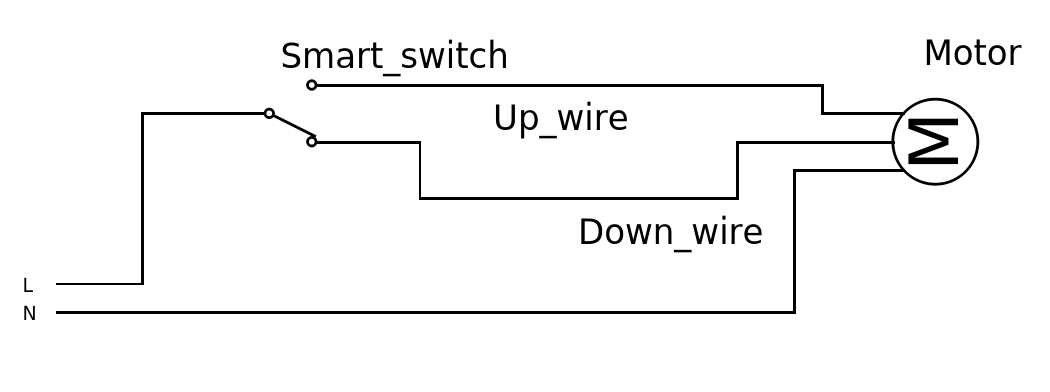
\includegraphics[width=\linewidth]{motor}
    				\caption{Motor activation \label{motor}}
  				\end{center}
				\end{figure}
%++++++++++++++++++++++++++++++++++++++++++++++++++++++++++++++++++++++++++++

\section{Failure handling}\label{failure_handling}
Failure handling is the most complex part of this system because we need to detect many things like broken actuators, broken sensors, 
network failures or to deal with a Central Unit crash.
\subsection{Sensors or actuators failures}
It is possible for the Central Unit to detect a sensor or actuator failure. 
% Je pense qu'on y arrive, mais il faudra préciser que pour chaque message envoyé, il faut le reconnaître en envoyant un message ACK/SYN
%But it is genrally hard to decide by a detection if a sensors is broken of if an actuator has a failure.
%We can take the following case as an example.
%Admit we want to detect a sunblind failure. Then we can take as 
\subsubsection{Sensors}
In general sensor failures are easy to detect because the small computer that aggregates its sensor values can detect that a sensor not sending values anymore. 
Different sensors behaviors as sensors degradation or skew sensors values can be detected via simple machine learning as computing mean and variance of sensor outputs and detect abnormal variations via a probabilist model.
After a sensor failure detection, the sensors send a message to the Central Unit. %c'est pas plutôt la petite unité computationnelle qui envoie le message si le senseur est down? Il faudra aussi traiter le cas où c'est cette unité computationnelle qui est down, mais le senseur toujours ok...
\begin{verbatim}
POST central_unit 
  <MESSAGE>
    <TYPE>failure</TYPE>
    <FROM>sensor_id</FROM>
    <CONTENT>failure_code</CONTENT>
  </MESSAGE>
\end{verbatim}
\subsubsection{Actuators} 
Actuator failures are harder to detect due to the fact that no value is directly return by an actuator.
But by inference one can easily detect some incoherence in the system.
For example if the room sensors returns a "dark" state for a room and a light is activated in the room. Then the light bulb might be broken.
In that case no message is passed as the central unit itself compute this failure.
\subsection{Smart switch failure}
The failure of a smart switch can lead to very problematic behavior such as the total incapacity of making actuators work.
This will lead to not beeing able to use the lights anymore or to open the sunblinds anymore.
The main idea here is to let the user have a control on the switches physically with a standard switch button.
The problem still exists if the switches are part of a "shema 3" for example. The users need to activate all the switches to be able to light a bulb on such a configuration.
But this gives a quite acceptable solution until the switch replacement.

\subsection{Central Unit failure}
This part is the most critical failure possible.
Our central unit is the main component of our system and thus a single point of failure.
Allowing the user to have little physical control on the switches is a good solution to begin with.
Another additional feature would be to add a little portable computer as a tablet at the entrance of each appartment 
to let the user bypass the Central Unit messages and to control the whole appartment with a specifically designed application.
It could also remotly reboot the Central Unit if needed and control the patches installation.
This little tablet could also display the errors of the system and allow a more easy way fix to the failure.
All user parameters could also be stored on this computer as backup.
This would more or less give us a structure with two points of failure (the central unit and the portable device) which is much more robust.

\subsection{Failure notification}
An user-firendly feature would be to notify the users in case of failure. This can easily be done via the web interface itself as suggested in Figure \ref{mockup} or via other means such as SMS or email services.

\section{Conclusion}

% Hard to produce at the End
% We tried to do as cheep as possible but it is clearly not possible if we want a reliable system
% It is full extensible because of the central unit. We simply need to add more context and inference related.
% The web interface can lead to more user-friendly features such as a Facebook look-like timeline to monitor the house activity.
% We can make use of more machine-learning and thus make the house learn a bit about the users and their habits.
% Machine learning could be useful in temparature management for example (lower the temp when users are usually not there).



\section{Acknowledgments}



\nocite{*}
% The following two commands are all you need in the
% initial runs of your .tex file to
% produce the bibliography for the citations in your paper.
\bibliographystyle{abbrv}
\bibliography{sigproc}  % sigproc.bib is the name of the Bibliography in this case

\end{document}
